\subsection{Model Animation}
\label{sec:MA}

To answer Challenge C2, it is important to design the MA framework with
the idea of reuse at its core. One possible approach is to separate two
things: the basic blocks defining animations \emph{effects} that may be combined
into comprehensive Model Animation Units (UAs), from the way they are organised
and scheduled to build complex animations. The approach we propose is similar
to the de-/reconstruction of MTLs described by \citet{J:SyrianiVangheluwe:2013}:
the idea is to capture the most basic animation effects, and offer powerful 
mechanisms to combine them, resulting in the ability to effectively specify any
kind of animation. We quickly discuss basic effects before describing two
approaches for scheduling.



\subsubsection{UA Effects}
\label{sec:MA-Effects}

Effects may be roughly classified into four categories, depending on the features
they act on:
\begin{description}
   \item[Creation] effects bring an element into a diagram in various ways, e.g. by
   simply making it appear at the right position, or by ``zooming'' it in, i.e.
   starting from a small size until reaching its regular size, while preserving 
   the element's proportions.
   
   \item[Deletion] effects remove an elements from a diagram, e.g. by making it
   disappear, or by ``zooming'' it out. 
   
   \item[Action] effects update one, or several of the visual features of an
   element, e.g. the color, size, etc. of a text, a shape or a connector.
   
   \item[Path Motion] effects move an element along a predefined path, e.g. a
   straight or curved line, or the line represented by a connector.
\end{description}
We expect that most of the MAs would make use of a small set of basic effects. 
These effects could be organised into libraries and potentially exchanged among
MA specialists, but their reuse across different platforms may be hindered by how
effects are highly dependent on the way the graphical components of the CS are
defined.

As illustrative examples, \textsf{PM.3}, \textsf{FSM.1.2} and \textsf{PN.1} and \textsf{PN.2}
all falls into the \emph{Action} effects category, because only the graphical 
features (or values) of the score label, the \textsf{Letter} and the color of the
\textsf{Arc}(s) are modified. \autoref{fig:FSM_M} graphically illustrates,
in the middle, an possible way to realise a \emph{Path Motion} effect. Finally,
\emph{Creation} and \emph{Deletion} effects are combined to realise a complex 
animation in \textsf{FSM.2.1}, \textsf{PM.1} and \textsf{PN.3.2}. 

\subsubsection{UA Scheduling}
\label{sec:MA-Scheduling}

\begin{figure}[t]%
   \centering
   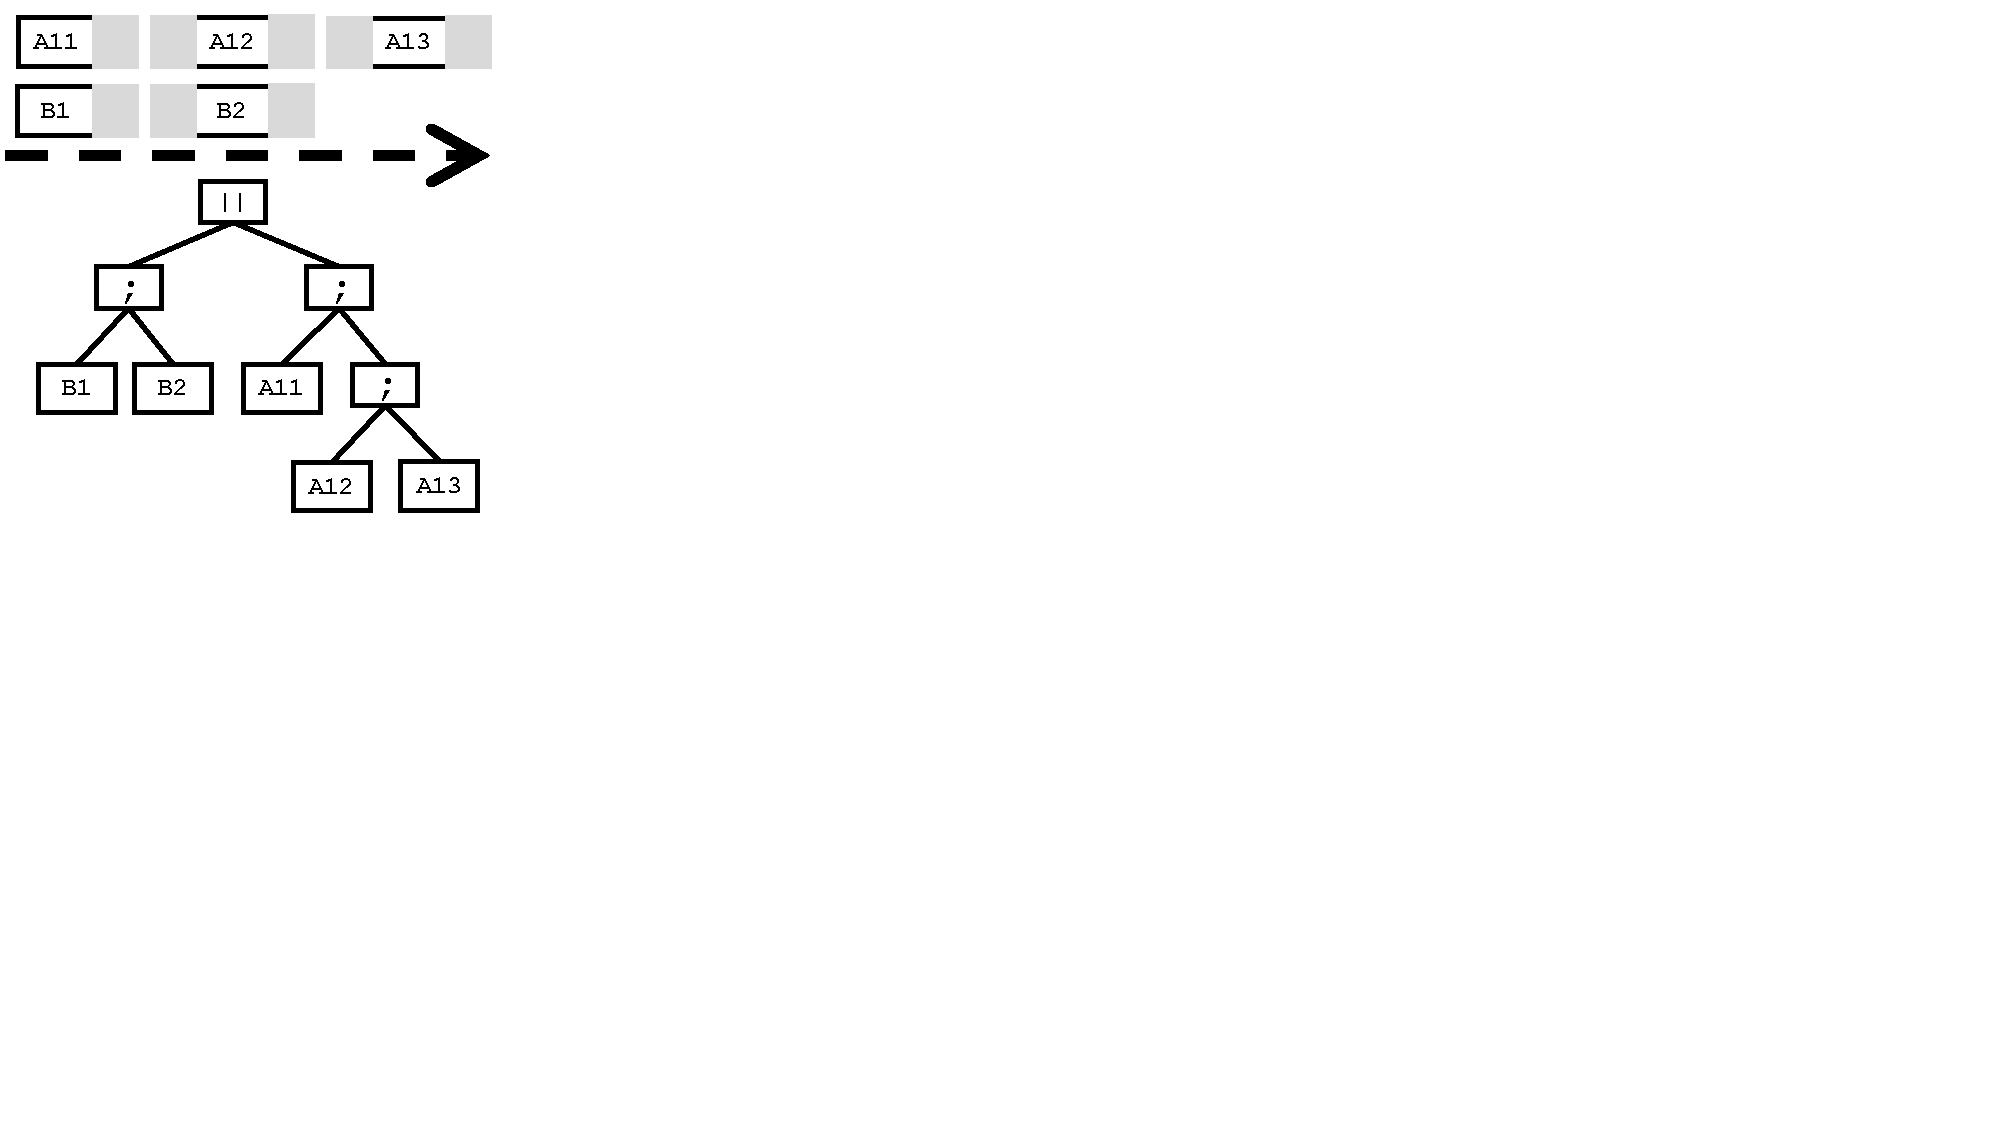
\includegraphics[width=\columnwidth,clip, trim=0cm 10cm 25cm 0.2cm]{UAScheduling}%
   \caption{On top, scheduling is realised with \emph{embedding}: each AU has 
   pre- (except the first) and post-conditions, represented as grey blocks attached 
   before and after the AU. On bottom, the same animations but with UAs organised with
   two combinators: \texttt{\textbf{||}} for parallel, and \texttt{\textbf{;}} for
   sequential combinations (the temporal details are omitted).
   }%
   \label{fig:UA-Schedule}%
\end{figure}

Although theoretically equivalent, two approaches are possible for realising
this requirement.
\begin{description}
   \item[Embedding the scheduling \emph{inside} the UAs] As suggested in 
   \autoref{fig:UA-Schedule} (left), each UA is extended with pre- and 
   post-conditions. A precondition indicates how an UA starts relatively to the 
   previous one (at the same time, after, or delayed by a given time); while a
   postcondition would define whether the UA is repeated (and how many times).
   
   \item[Define \emph{combinators outside} of UAs] Another approach, suggested
   in \autoref{fig:UA-Schedule} (right) is to provide explicit \emph{combination}
   operators (aka. \emph{combinators}) that would take as operands UAs. Combinators
   similar to the previous case may be defined: sequencers with a possible delay,
   repetitors, and parallelisation. 
\end{description}
The second approach may seem more familiar to MA designers with a programming 
background, because the combinators approach proposes constructions similar to
what is available in GPLs. However, the first approach may be more compact visually,
and familiar for MA designers accustomed to slideshow tools (the most popular and
mainstream ones being Microsoft Powerpoint, Apple Keynote and Google Slides, among
a plethora of other dedicated tools, many of which only existing online).

Note that both approaches may concurrently exist, allowing MA designers to choose
the most appropriate approach for specifying their MA. It is left as future work
to study under which conditions they may coexist (if possible at all), and to 
identify when and how each presents more benefits than the other.
